\section{Data Quality Evaluation}
\subsection{Automatic Quality Evaluation}

% 和其他方法比较complexity score和quality score
\begin{figure}[pos=htbp]
\centering
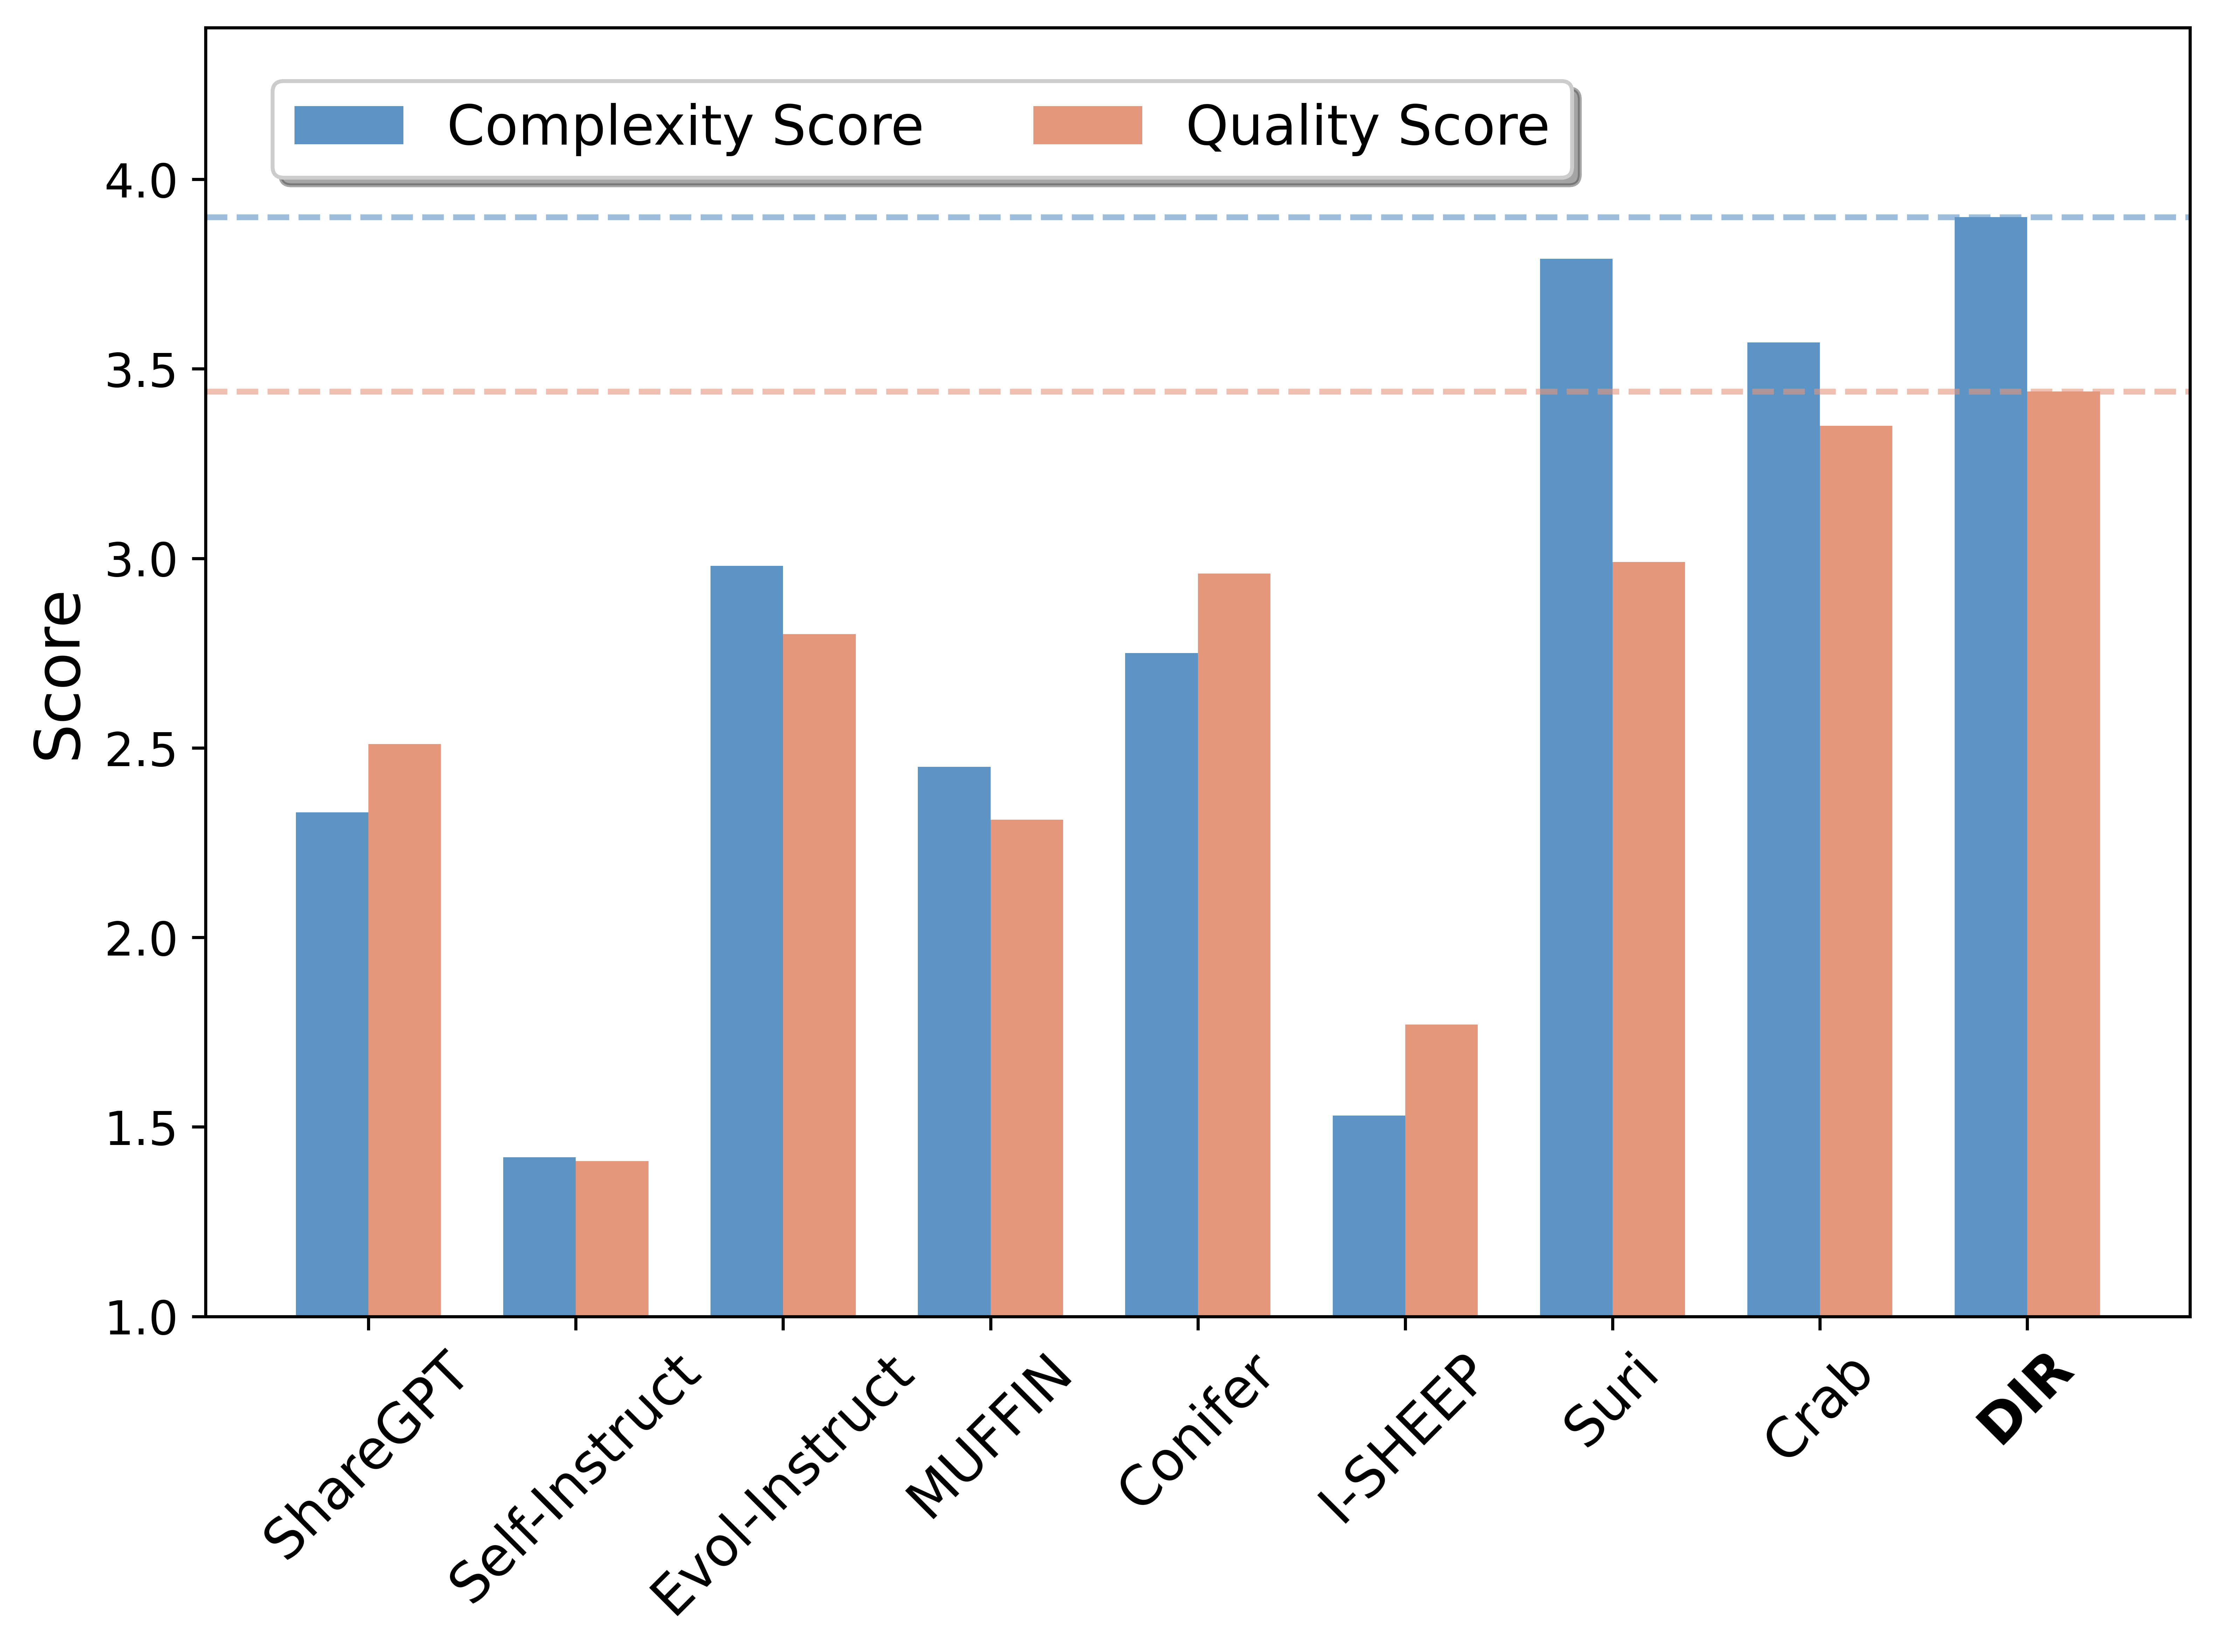
\includegraphics[width=0.9\linewidth]
{source/complexity_scores.png}
\caption{Averaged complexity and quality scores on different datasets.}
\label{figure:complexity_scores}
\end{figure}


% 轮次间的指令长度变化情况，complexity score和quality score变化情况
\begin{figure}[pos=htbp]
\centering
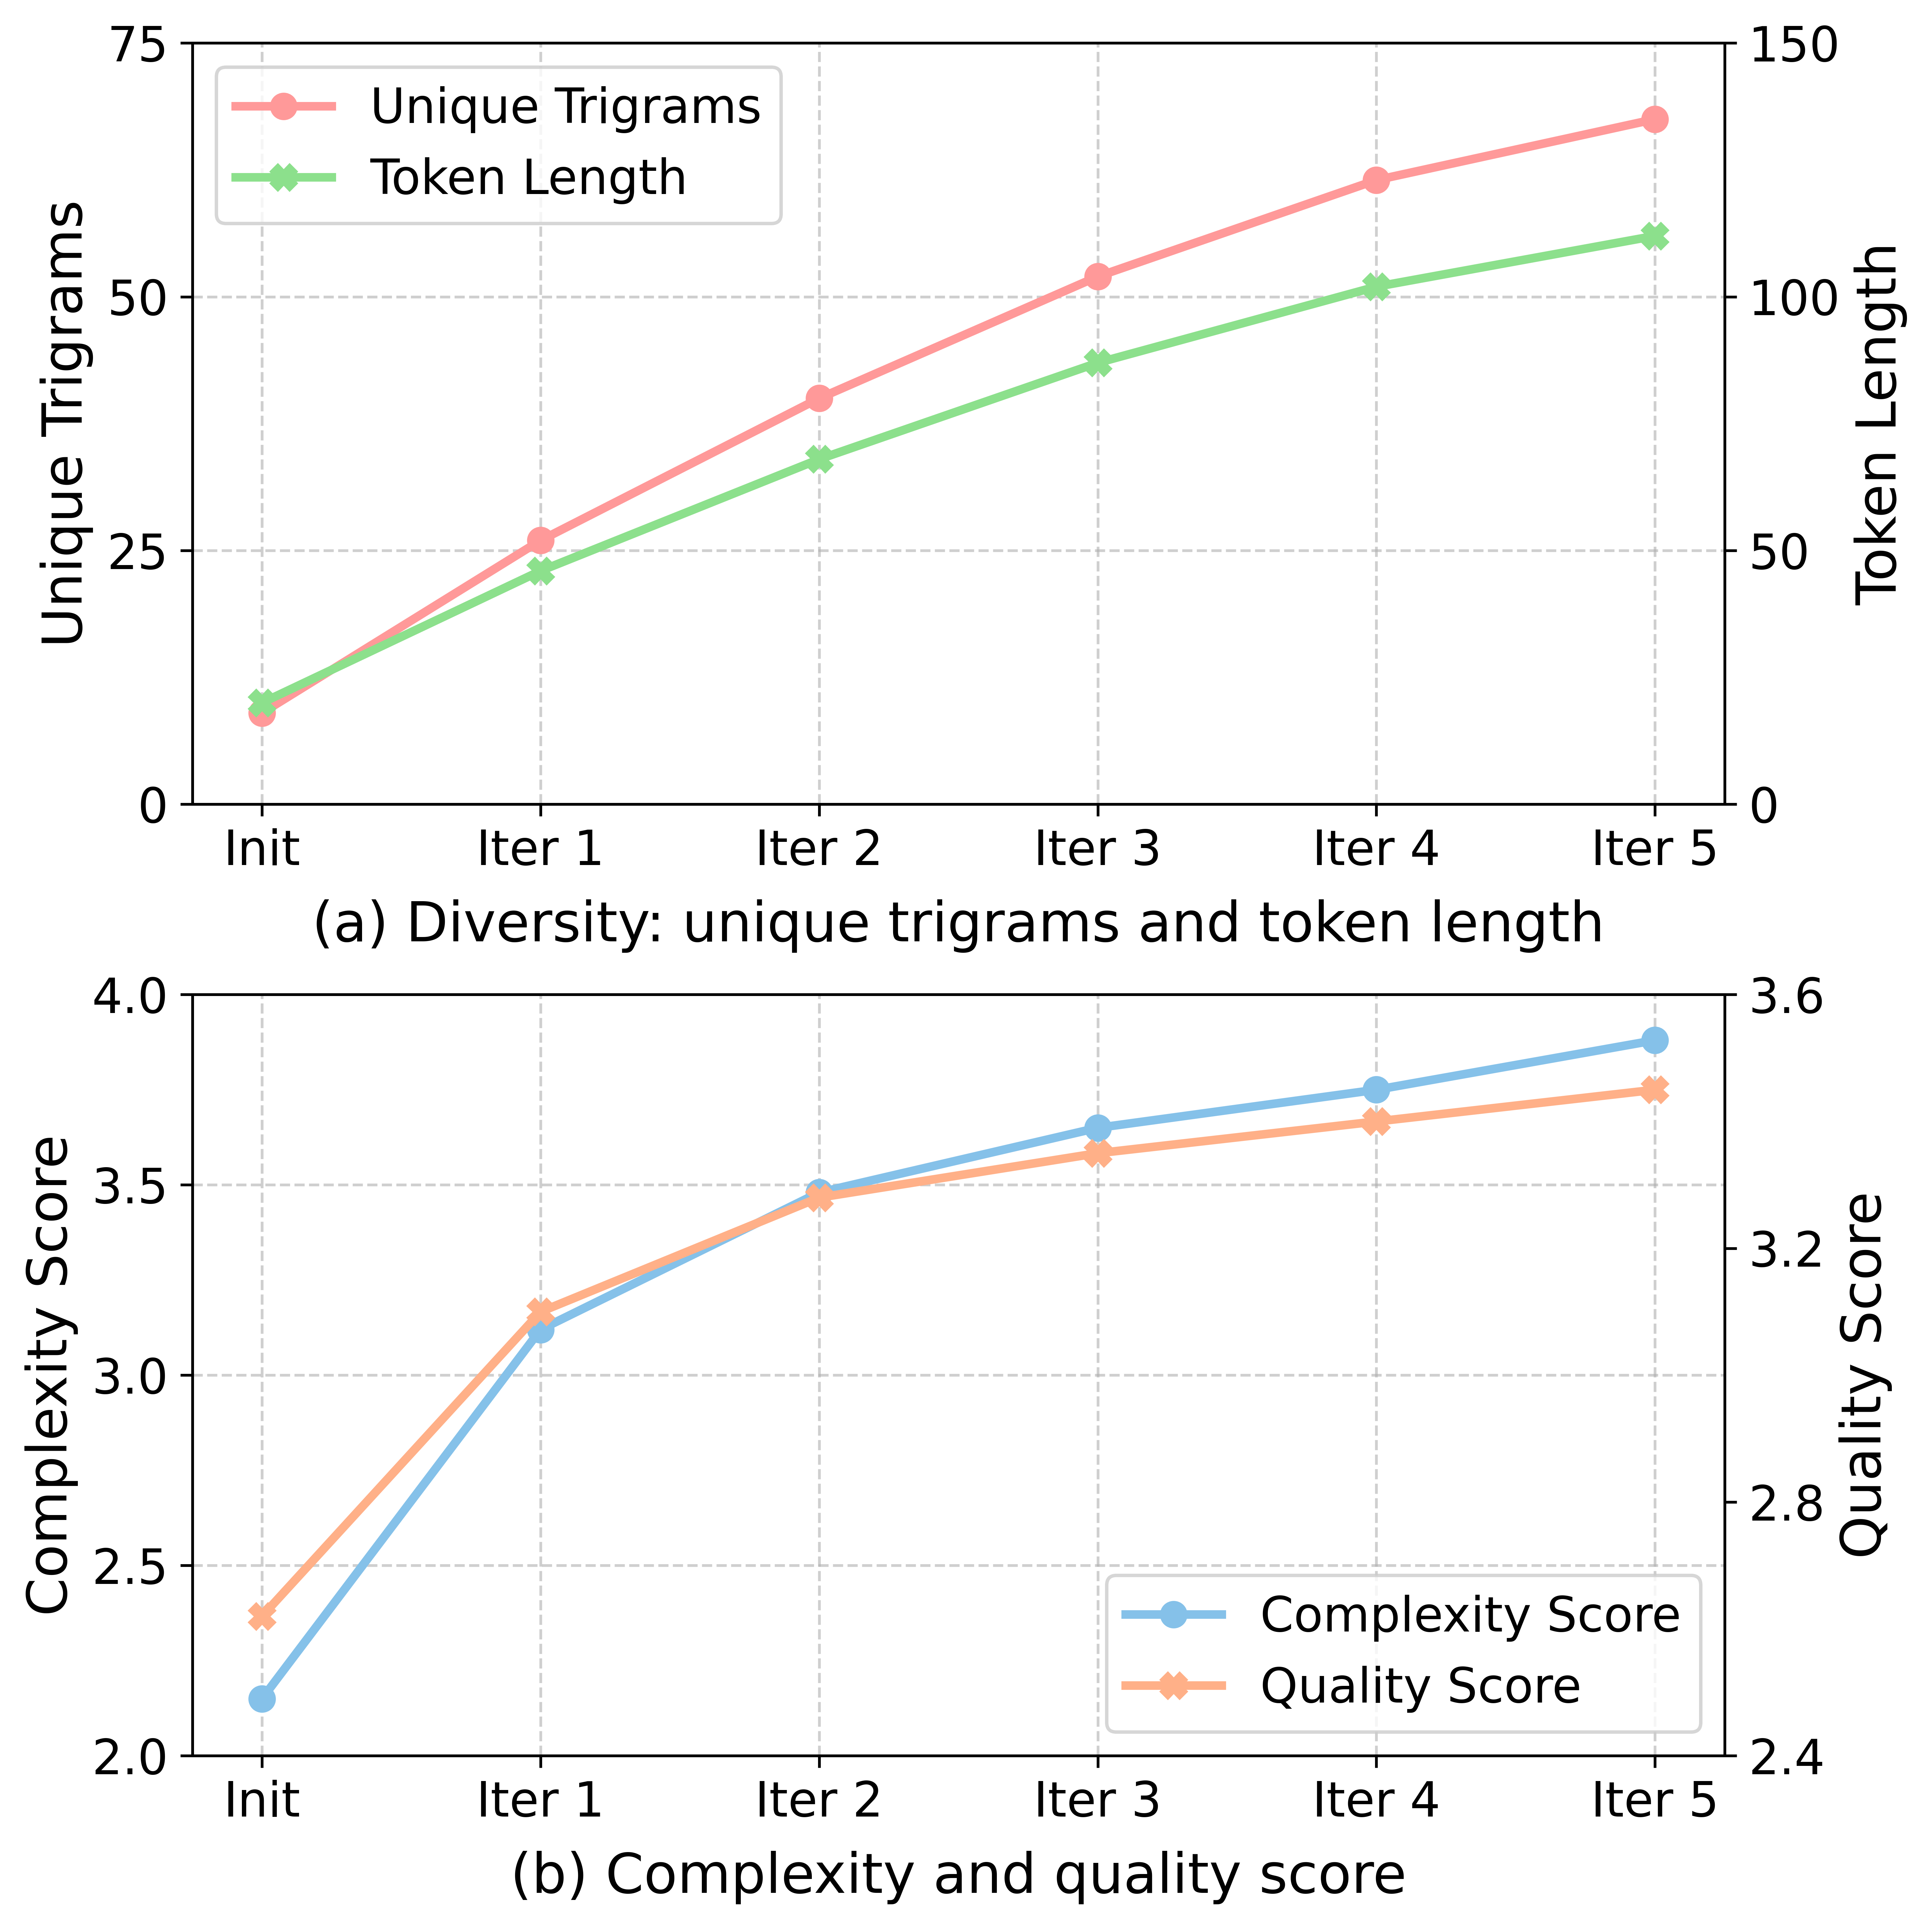
\includegraphics[width=0.95\linewidth]{source/instruction_and_complexity.png}
\caption{Variation of quality indicators of DIR generated data across iterations. \textit{Init} represents initial instructions generated by IIG.}
\label{figure:instruction_and_complexity}
\end{figure}

% To investigate the effect of iterative refinement, we analyze the variation of average unique trigrams and token lengths across iterations in Figure \ref{figure:instruction_and_complexity}(a). The results demonstrate consistent increases in both instruction length and unique trigrams, indicating that newly added constraints are diverse rather than mere repetition. Furthermore, Figure \ref{figure:instruction_and_complexity}(b) displays the evolution of complexity and quality scores throughout the iterations, showing steady improvement of data quality as the iterations progress.

To quantitatively assess data quality, we employed the DEITA scorer \citep{liu2024Deita}, which leverages an LLM-based framework to evaluate instruction complexity and the overall quality of instruction-response pairs. As shown in Figure \ref{figure:complexity_scores}, our approach significantly outperforms previous instruction datasets in terms of both complexity and quality scores. Notably, our method shows marginal improvements over automatic back-translation approaches like Suri and Crab, despite their use of high-quality seed datasets (e.g., Alpaca-GPT4 for Crab) and advanced models (e.g., GPT-4-turbo for Suri). These results validate the effectiveness of our data synthesis strategy.

Furthermore, we investigated the impact of the iterative refinement process by tracking key quality indicators over five iterations (Figure \ref{figure:instruction_and_complexity}). As shown in Figure \ref{figure:instruction_and_complexity}(a), both average token length and the count of unique trigrams exhibit a steady, near-linear increase. This confirms that each iteration introduces novel, non-redundant constraints, thereby enhancing constraint diversity rather than merely repetition. Correspondingly, Figure \ref{figure:instruction_and_complexity}(b) shows that complexity and quality scores improve monotonically. Notably, while the most substantial gains occur in the initial iterations, the continued upward trend across all metrics confirms the efficacy of the iterative cycle in progressively elevating data sophistication.

\subsection{Human Preference Evaluation}

To complement our automated quality evaluation metrics, we conducted a blind, pairwise human evaluation to compare instructions generated by our DIR framework against three representative baselines: \textbf{ShareGPT}, \textbf{Conifer} \citep{sun2024conifer} and \textbf{Crab} \citep{qi2024constraint}. To ensure a fair and controlled comparison, each instruction pair was generated from identical source corpora. From each baseline, 100 samples were randomly selected for side-by-side comparison. Three annotators with Master's degrees and proficiency in NLP were recruited. The annotators were asked to select a winner for each instruction pair based on three evaluation criteria: \textit{Instruction Complexity}, \textit{Instruction Clarity}, and \textit{Overall Preference}. The final results, determined by majority vote, are presented in Table \ref{table:human_eval_results}.

\begin{table}[!t]
\centering
\caption{Pairwise human evaluation for data quality.}
\renewcommand{\arraystretch}{0.95}
\resizebox{0.48\textwidth}{!}{
\begin{tabular}{cl|ccc}
\toprule
\textbf{Comparison} & \textbf{Evaluation Criterion} & \textbf{Win} & \textbf{Lose} & \textbf{Tie} \\
\midrule
\multirow{3}{*}{\makecell[c]{DIR \\ vs. \\ ShareGPT}} & Instruction Complexity & \textbf{66.0} & 30.0 & 4.0 \\
& Instruction Clarity & \textbf{58.0} & 33.0 & 9.0 \\
& Overall Preference & \textbf{60.0} & 29.0 & 11.0 \\
\midrule
\multirow{3}{*}{\makecell[c]{DIR \\ vs. \\ Conifer}} & Instruction Complexity & \textbf{69.0} & 21.0 & 10.0 \\
& Instruction Clarity & \textbf{67.0} & 23.0 & 10.0 \\
& Overall Preference & \textbf{68.0} & 23.0 & 9.0 \\
\midrule
\multirow{3}{*}{\makecell[c]{DIR \\ vs. \\ Crab}} & Instruction Complexity & \textbf{70.0} & 23.0 & 7.0 \\
& Instruction Clarity & \textbf{67.0} & 27.0 & 6.0 \\
& Overall Preference & \textbf{67.0} & 21.0 & 12.0 \\
\bottomrule
\end{tabular}}
\label{table:human_eval_results}
\end{table}

\begin{table}[!t]
\centering
\renewcommand{\arraystretch}{1.0}
\caption{Inter-annotator agreement for pairwise human evaluation.}
\resizebox{0.32\textwidth}{!}{
\begin{tabular}{lc}
\toprule
\textbf{Comparison} & \textbf{Fleiss' Kappa (\%)} \\
\midrule
DIR vs. ShareGPT & 82.82 \\
DIR vs. Conifer  & 83.34 \\
DIR vs. Crab     & 80.47 \\
\bottomrule
\end{tabular}}
\label{table:human_eval_kappa}
\end{table}

As can be seen, the results reveal an overwhelming preference for instructions generated by our DIR framework across all criteria. This study provides human-centric evidence that the instructions generated by DIR are not only more complex but also more aligned with human preference than other instruction synthesis methods. 

To ensure the reliability of these judgments, we also calculated the inter-annotator agreement using Fleiss' Kappa \citep{fleiss1971measuring}. As shown in Table \ref{table:human_eval_kappa}, the high agreement scores confirm the consistency and validity of our human evaluation process.